\documentclass[11pt]{article}

\usepackage{hyperref}
\usepackage{graphicx}
\usepackage[nottoc]{tocbibind}
\usepackage{amsmath}

\begin{document}


\section{Introduction}

In the 2018-2019 sessions nearly 200,000 bills were introduced in state legislatures in the United States. Only 

\section{Related Work}

\begin{itemize}
  \item Legislative Data
  \item Text Classification with Metadata
\end{itemize}


\subsection{Quantitative Political Science}

Quantitative Political Scientists have been analyzing legisltive data and it's behavior for years. To date most studies in the US have focused on Federal
legislation given the breadth of high quality datasets available. The methods roughly track the advances in natural laguage processing over the years.

Gerrish and Blei (2011)\cite{gerrish2011predicting} construct a topic model given bill text and individual legislator's votes and use supervised methods to explore how
topics relate to voting paterns.

Nay (2017) \cite{nay2017predicting} Takes Federal legislation and predicts enactment using word vectors, gradient boosting, and ensemble stacking. A dozen features
are constructed out of bill sponsors, committee data, and subject. Various combinations of text, metadata, and text plus metadata are analysed 

\subsection{Text Classification with metadata}

Zhang etal. (2021)\cite{zhang2021match}

\section{Data and Models}

\subsection{Data}

We were provided data from a private company \href{https://govhawk.com/}{GovHawk} that collects state and federal legislative data in realtime and 
sells subscriptions to parties interested in the legislative process. The data encompasses the 2018-2019 legislative session for upper and lower house in
every state (nebraska has one). Substantial amount of data on individual votes and party identification of congresspeople was provided but was not complete for
every state. The data was processed into the following features for use in modeling.

\textbf{Bill Text} - The raw text provided by each legislature is in legal markup and contains a large amount of extra content not related to specifics of the bill. 
Headers, footers, and boilerplate language were removed. References to other legislation, section/subsection language, and all numbers and extraneous symbols were removed.
The text was made into lower case. The remaining text is a good faith effort at the natural language of the bill. See appendix for an example (TODO).

\textbf{Revision Number} - Bills go through a natural revision process and the current number of revisions is available at prediction time and thus has relevant information. 
Inclusion of all revisions of a bill would contribute to overfitting of a model. Therefore, for each bill we select one revision at random and include it in our dataset.
This reduces the number of observations from over 600,000 to around 200,000.

\textbf{Partisan Lean} - The liberal/conservate membership of each legislature was calculated and coded as a continuous variable from 0.0 to 1.0
 where 0.0 is an all conservative legislature, 0.5 is an even split, and 1.0 is an all liberal legislature. The intuition for this feature is that an 
 NLP model should upweight the passage of "liberal" legislation in a liberal legislature and downweight it in a conservative one. To the extent possible this was
 derived from available metadata, where not the values were filled in from wikipedia.

\textbf{Session-Chamber} - A categorical variable encoding the legislature, session pair from the dataset. Some legislature's sessions comprise multiple years and bills
carry over from one to the next. Texas meets every two years. In all there are 133 categories that are one-hot encoded.

\textbf{Passage} - A two class (0/1) variable indicating whether the legislation passed the specific legislature. 

\textbf{Signed} - A two class (0/1) variable indicating whether the legislation passed by both legislatures and the executive.


\begin{itemize}
  \item \textbf{TODOs}
  \item Verify time frame for state legislatures for sessions ? to ?.
  \item Example bill cleaning in an appendix.

\end{itemize}

\subsection{Baseline Models}

\subsection{Bag of Words Models}

\subsection{Transformers}

Transformers revolutionized natural language processing with the invention of the attention mechanism \cite{DBLP:journals/corr/VaswaniSPUJGKP17}.

$$ Attention(Q,K,V) = Softmax(\frac{QK^T}{\sqrt{d_k}})V $$

For a single token embedding (a vector) the \textit{query (Q)} is a vector: Attention(vector, matrix, matrix) \rightarrow vector.

$$Attention(query, Key, Value) = Softmax(query * Key^T) * Value$$

This operation is parallelizable and the algorithm will 



Huggingface library \cite{DBLP:journals/corr/abs-1910-03771}

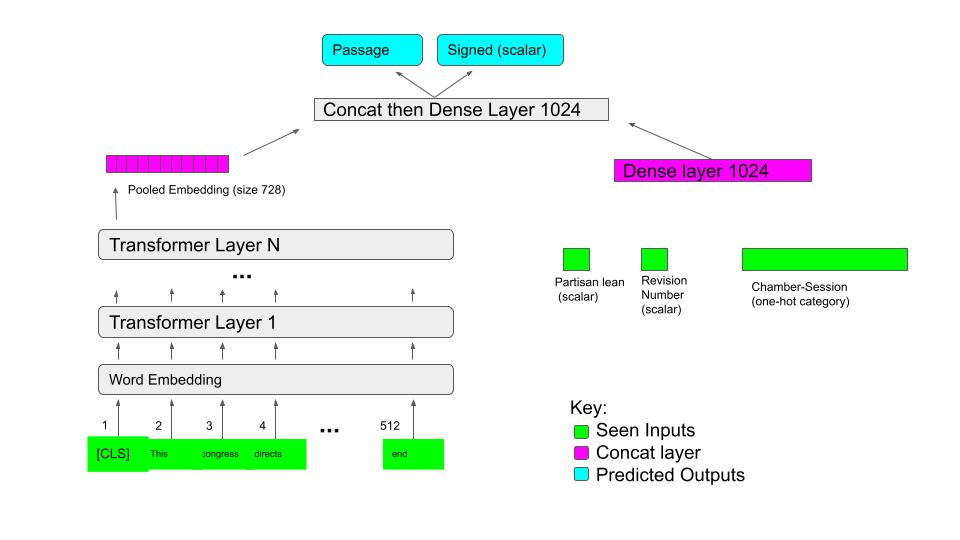
\includegraphics[width=150mm]{network_architecture.jpg}
%\caption{Figure X - Network Architecture}

\section{Results}

\begin{tabular}{ l  c  c  c}
 Model & AUC & Precision & Recall  \\
 \hline
 \textbf{Metadata Only} & & & \\
\hspace{3mm}Logistic Regression & 0.871 & 0.69 & 0.33 \\
\hspace{3mm}Catboost  & 0.888 & 0.68 & 0.43 \\
\hspace{3mm} Dense Neural Network & 0.883 &  0.69 & 0.39 \\
\hline
\textbf{BoW Text Models} & & & \\
\hspace{3mm}Logistic Regression with LDA & 0.883 & 0.71 & 0.35 \\
\hspace{3mm}CatBoost with LDA & 0.912 & 0.74 & 0.55 \\ 
\hline
\textbf{Transformer with Metadata combinations} & & & \\
\hspace{3mm}Only Metadata & 0.883 & 0.69 & 0.39 \\
\hspace{3mm}Text Only & & & \\
\hspace{3mm}Text, Revision Number, Legislature & & & \\
\hspace{3mm}Text and Partisan Lean & & & \\
\hspace{3mm}Text and All Metadata & \textbf{ 0.936 }& \textbf{0.81} & \textbf{0.55} \\
\hline
\textbf{Different Transformers (all metadata)} & & & \\
\hspace{3mm}DistilBert (128 tokens) (2 epochs fine-tune) & \textbf{ 0.936 }& \textbf{0.81} & \textbf{0.55} \\
\hspace{3mm}DistilBert (512 tokens)  &  & & \\
\hspace{3mm}Bert (128 tokens) &  & & \\
\hspace{3mm}Bert (512 tokens)  &  & & \\
\hspace{3mm}DistilBert (512 tokens) &  & & \\
\hline
\textbf{Different Transformers (all metadata)} & & & \\
\hspace{3mm}DistilBert (512 tokens) Feature Selector plus Catboost&  & & \\

\end{tabular}

\vspace{3mm}

[1] Dense Neural Network is precisely the same inputs and dense layer as used inside the transformer-based models and is 
included as to measure the gain from transformers. 

\subsection{Partisanship in Legislation via Ablation Analysis}

\begin{itemize}
  \item Partisan Lean and quantifying partisanship in a bill.
  \item Revision number and predicting left-out revisions.
\end{itemize}

\section{Summary}




\section{Bibliography Todo}

\begin{itemize}
  \item \textbf{papers to digest}
  \item Categorical Metadata Representation for Customized Text Classification  https://transacl.org/ojs/index.php/tacl/article/view/1619
  \item Large Scale Legal Text Classification Using Transformer Models  https://arxiv.org/abs/2010.12871
\end{itemize}


\bibliography{deep_legis}
\bibliographystyle{amsplain}

\end{document}